\documentclass[11pt,letterpaper]{article}
%% Coverpage Packs
\usepackage{wallpaper}

%%Query packs
\usepackage[utf8]{inputenc}
\usepackage{amsmath}
\usepackage{amsfonts}
\usepackage{amssymb}
\usepackage{url}
\usepackage{xcolor}
\usepackage{fullpage}
\usepackage{listings}
\usepackage{mathtools}
\usepackage{enumitem}
\usepackage{bm}
\usepackage{fixltx2e}
\usepackage{hyperref}
\usepackage{array}
\usepackage{multirow}
\usepackage{longtable}

\lstset{
	basicstyle=\ttfamily,
	columns=fullflexible,
	breaklines=true,
	postbreak=\mbox{\textcolor{red}{$\hookrightarrow$}\space},
}
\setlength\parindent{24pt}

%%Graphics packs
\usepackage{ulem}
\usepackage{geometry, tikz}
  \usepackage{graphicx}
\usetikzlibrary{shapes,shadows,arrows.meta}
\geometry{
    a4paper,
    total={170mm,257mm},
    left=20mm,right=20mm,
    top=20mm,
}

%%Assumption/Constraint Packs
\usepackage{enumitem}

\title{Comp353 Project Report}
\author{Kai Nicoll-Griffith[40012407], Stephen Prizio[40001739], \\Giovanni Gebran[40018637], Nizar Belhassan[27519443]\\\\\bf{Team kzc353\_4}}

\begin{document}
	
	

	\begin{titlepage}
\iffalse
\tikz[remember picture,overlay] \node[opacity=1.0,inner sep=0pt] at (current page.center){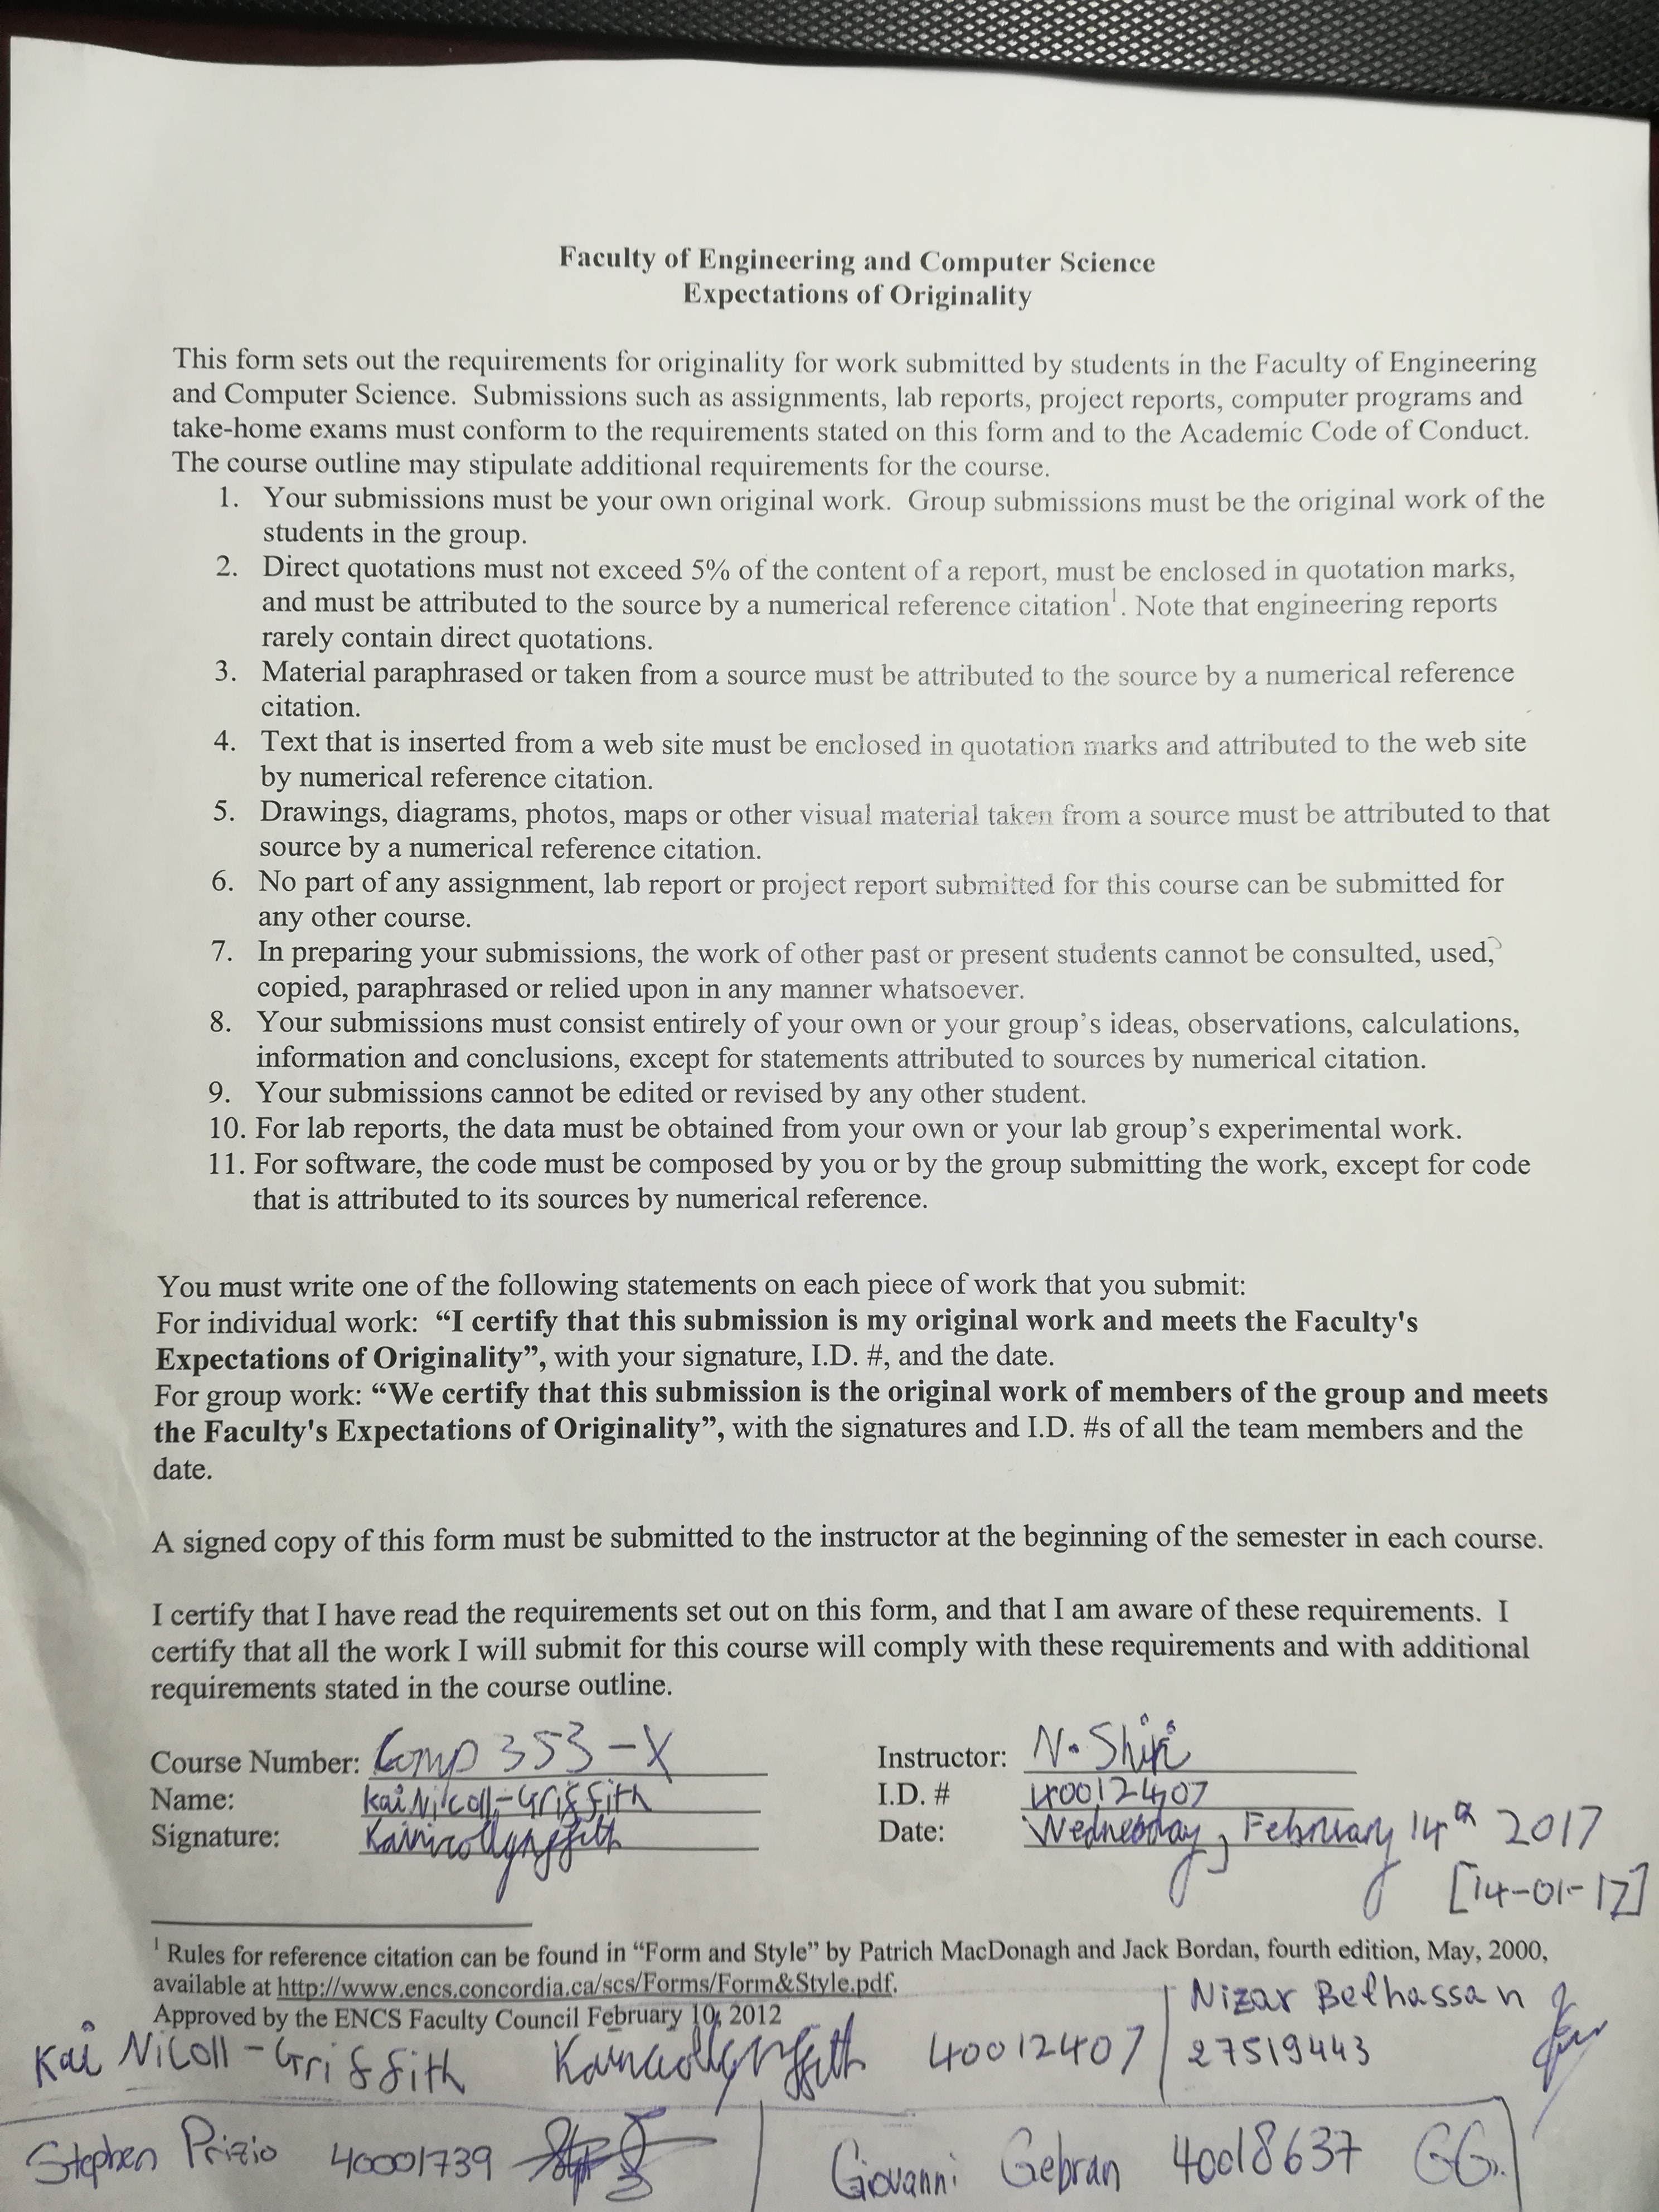
\includegraphics[width=\paperwidth,height=\paperheight]{originality.jpg}};
\fi
\end{titlepage}
	
		\maketitle
		\newcommand{\graphicwidth}{18.5cm}
	\section{Entity Relationship Diagram}
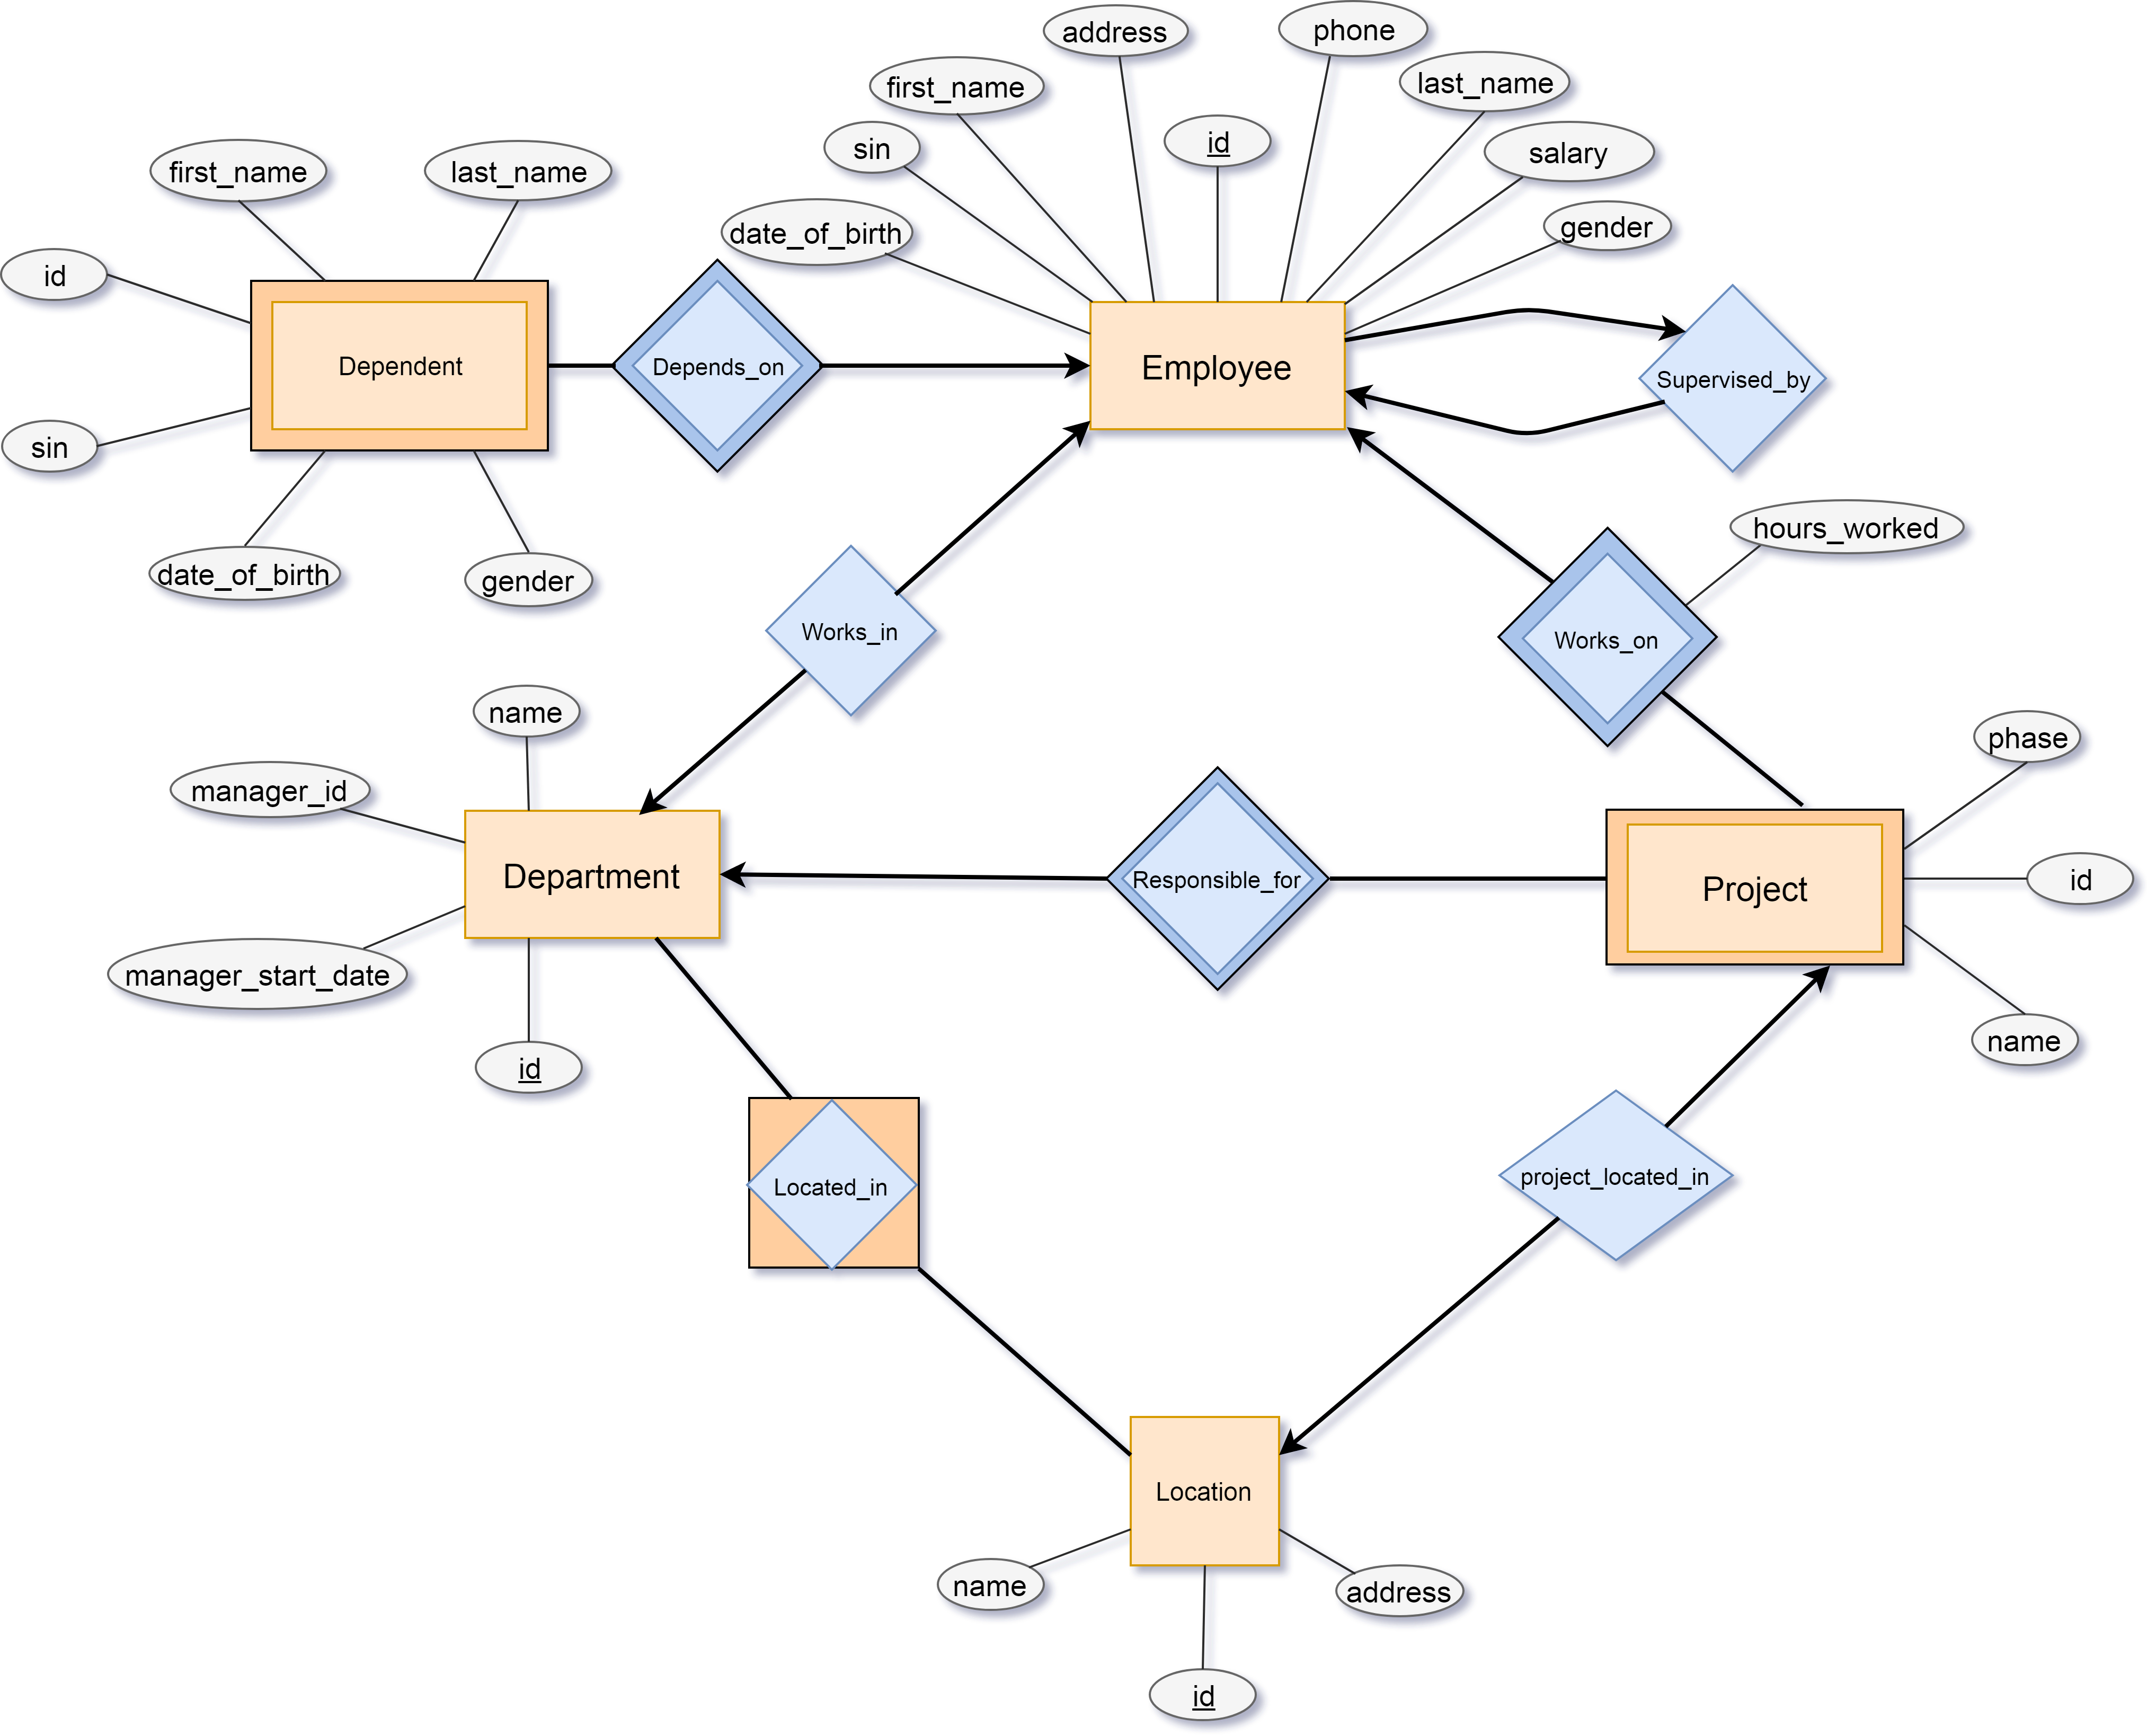
\includegraphics[width=\graphicwidth]{erd.png}
	\section{Reasonable Assumptions and Constraints}
	
In the COMPANY database There are three primary categories of entity from which more complex entities are defined. These are:
\begin{enumerate}[]
	\item departments, 
	\item employees,
	\item projects,
\end{enumerate}

Since there will need to be multiple links to better define this entity and negative ids are unsightly, departments are identified with a primary key ID which is an unsigned integer value with no auto increment. To easily identify the departments for employees, departments also have a unique name to be identified with. Since departments have people to look after, a manager employee manages the department. Managers are determined by an employee id which is a foreign key against the employee table and to record the date he starts is an attribute manager\_start\_date.
Both the manager\_id and manager\_start\_date are given the opportunity to be null since it is not always true that a department needs a manager. Small groups could potentially self manage if that is the policy of the company.\\

An Employee entity is a record of who a person within the company database is. Within it there are is no opportunity for optional parameters since it is assumed that a company needs to keep accurate track of everyone within it and null values would encourage poor data management practice of the company. Date of birth is required to keep track of retirement and phone numbers are an item everyone should have. An Employee has an unsigned integer ID, first\_name, last\_name, sin integer(unique due to nature of the SIN), a date of birth(date data type), an address, a phone number(char to enforce field size), an hourly salary(a 5,2 decimal datatype), a gender defined by one character and a linking department id integer for where the employee works. Unless otherwise noted, all datatypes are a varchar. The linking id is a foreign key that can not be null. An employee must work for a department.\\

A project is an item that is worked on by employees. It is assumed that multi-department projects are possible and is therefore given no firm and direct relation to a department within the tables of employee or department. However, it is assumed to be important that a project is given a firm location in where it is based and is therefore given a location\_id tying it to a specific location. It is identified by an unsigned integer ID to reference it(the primary key), a unique an mandatory name for employees to recognize it, and a location(unsigned integer location\_id) where it is worked on within the company. A location is a foreign key against the location entity. None of these attributes may be null as they are required to properly identify a unique project. Also included is a not null phase which keeps track of the progress of each individual project within the COMPANY database since it is assumed that keeping track of all project progress would be very difficult without a database solution.\\

These three main entity sets then are enhanced by the entity sets of:
\begin{enumerate}[]
	\item dependent 
	\item location
\end{enumerate}
And the role relation:
\begin{enumerate}[]
	\item role 
\end{enumerate}
A dependent is an entity that enhances the information of an employee by providing him with insurance information that the company might need to use. As it is vital information that has potential legal importance none of these fields may be null. A dependent has a primary unsigned integer ID to identify it and within it is a SIN as an unsigned integer, the foreign key employee\_id is needed to link the dependent to an employee. Since multiple employees may have with the same dependent the SIN can not be unique for this table. Also necicary for the dependent are the not null attributes of first name, last name, date of birth(date datatype) and a single character gender.  Unless otherwise noted, all datatypes are a varchar. \\

A location identifies where projects and departments are done. It is a list of possible locations where employees report their work to. These locations are identified by an unsigned integer, an optional name which is assumed to be used for employee convenience and an address which is used for more direct positioning and referencing. The name is a varchar, while the address is a medium text since it is assumed that the address could be as specific as country down to room number if the company so wishes.\\

The relationship of role helps to give more information the possible positions of importance an employee can have with his fellow employees. Since this table just defines the role of an employee against employee it does not handle department managers. It is assumed that this relation is solely used to show the hierarchy of employees within the company. It contains both unsigned and not null employee id to recognize the employee who is supervised by the supervisor\_id. Since our assumption is that an employee should only supervise one person, that he may be supervised by someone else and that he may not have a supervisor at all the employee \_id is a primary key enforcing uniqueness and no double counting, while the supervisor\_id is a default null value implying one is unsupervised which could be a possibility. This means an employee may both supervise and be supervised as defined by the role in relation.\\

Finally the assumptions on the relations bellow is that they create the connections between entity sets. These are:
\begin{enumerate}[]
	\item works\_on
	\item responsible\_for
	\item located\_in
\end{enumerate}
It's assumed one employee may work on many projects therefore this table solely uses foreign keys against the project and employee tables that may not be null. Since it is assumed to be important that an employee also logs the number of hours worked on projects(likely for financial and budgeting purposes) this relation also has a none-null default 0 value that keeps track of the hours.\\

Responsible\_for is used to connect the projects to the departments. It consists of unsigned foreign keys between the project and departments since the assumption is that multi department projects are possible.\\

Located\_in is needed due to the assumption that a department is not necessarily tied down to one location. It consists of unsigned foreign keys linking a location\_id to a department.

	\section{ER to Relation conversion }

\section {Normalization steps and assumptions}

\section{Implemented Functionalities}
	\subsection{Design Functionalities}
	The application makes use of the PHP 5.5.9 language due to it's reliable and simple functions for connecting with a MySQL database and forms to send queries to the database. In order to more easily input queries and build a front end system for users to interact with the database, Lavarel has been used to make development easier and have a more modern appearance.\\
	
	The company database consists of the tables: `department` allowing the storage of information on a department, `located\_in` providing the location of a department, a `location` table holding a set of locations the company operates in, `responsible\_for` linking the department to a multiple set of projects; `project` which covers details such as project completion and location, `works\_on` which indicates what employee works on what project; `Employee` which contains details on the staff of the company, `role` which specifies who is a supervisor and who is supervised, and `dependent` which is an employees dependents required for insurance purposes.
	Certain queries are used to allow the user to fulfill certain required functionalities.\\
	
	\subsection{Query Functionalities}
	24 Queries allow the system to select, update and add to the company database. These are in the form of .php filenames found in the source code folder.
	\subsubsection{delete\_department.php}
	DELETE FROM department WHERE department.id ='\$id'
	\subsubsection{get\_all\_projects\_for\_department.php}
	\subsubsection{get\_employee\_dependents.php}
	\subsubsection{get\_employee\_involved\_in\_least\_num\_of\_projects.php}
	\subsubsection{get\_employee\_involved\_in\_most\_num\_of\_projects.php}
	\subsubsection{get\_employee\_supervisor.php}
	\subsubsection{get\_employees\_who\_work\_on\_a\_project.php}
	\subsubsection{get\_hours\_worked\_employee.php}
	\subsubsection{get\_how\_much\_employee\_gets.php}
	\subsubsection{get\_project\_location.php}
	\subsubsection{get\_total\_hours\_worked\_for\_project.php}
	\subsubsection{get\_total\_pay\_for\_each\_project.php}
	\subsubsection{get\_how\_much\_employee\_gets.php}
	\subsubsection{get\_project\_location.php}
	\subsubsection{get\_total\_hours\_worked\_for\_project.php}
	\subsubsection{get\_total\_pay\_for\_each\_project.php}
	\subsubsection{insert\_department.php}
	\subsubsection{insert\_dependent.php}
	\subsubsection{insert\_employee.php}
	\subsubsection{insert\_located\_in.php}
	\subsubsection{insert\_location.php}
	\subsubsection{insert\_project.php}
	\subsubsection{insert\_responsible\_for.php}
	\subsubsection{insert\_role.php}
	\subsubsection{insert\_works\_on.php}
	
\section{contributions}
\subsection{Giovanni Gebran}
 \begin{itemize}
\item Database Design
\end{itemize}
\subsection{Nizar Belhassan}
 \begin{itemize}
\item Database Design
\item Majority of Queries
\end{itemize}
\subsection{Kai Nicoll-Griffith}
 \begin{itemize}
\item Database Design
\item Database Attribute Refinements
\item Report setup 
\item Report: ER Diagram
\item Report: Constraints and assumptions
\item Report: Functionalities
\end{itemize}
\subsection{Stephen Prizio}
 \begin{itemize}
	\item Database Design
	\item Front end Lazarel design
	\item SQL sample data and database 
	\item Minority of Queries
\end{itemize}
\end{document}
